\documentclass[a4paper, 11pt]{article}
\usepackage{fullpage}

\usepackage[utf8]{inputenc}
\usepackage[swedish]{babel}

\usepackage{amsmath}
\usepackage{amsfonts}
\usepackage{amssymb}
\usepackage{graphicx}
\usepackage{float}
\usepackage{listings}
\usepackage{multirow}
\usepackage{fontenc}

\usepackage[hidelinks]{hyperref}

\usepackage{titlesec}
\setcounter{secnumdepth}{4}

\usepackage[backend=biber,style=numeric,sorting=none]{biblatex}
\addbibresource{cites.bib}

\usepackage{caption}
\captionsetup[figure]{name=Figur}

\begin{document}

\begin{titlepage}
\newcommand{\HRule}{\rule{\linewidth}{0.5mm}}
\begin{center}

\textsc{\Large }\\[2.5cm]
\textsc{\LARGE Uppsala Universitet}\\[1.5cm] 

\HRule \\[0.3cm]
{ \huge \textup {Historiekunskapsspel med semiautomatisk frågehämtning och ett balanseringssystem för frågor}}\\[0.3cm]
\HRule \\[1.5cm]


\Large \textsc{Författare:}\\[0.5cm]
\end{center}
\begin{minipage}{0.4\textwidth}
\begin{flushleft} \large
\large \textup{Alfred Yrelin}\\
\large \textup{Alfred.Yrelin.2125@student.uu.se}\\
\large \textup{\textup{Inst. för informationsteknolog}}\\
\large \textup{\textup{Uppsala Universitet}}
\end{flushleft}
\end{minipage}
~ \hfill
\begin{minipage}{0.4\textwidth}
\begin{flushright} \large
\large \textup{Josef Svensson}\\
\large \textup{Josef.Svensson.8440@student.uu.se}\\
\large \textup{\textup{Inst. för informationsteknologi}}\\
\large \textup{\textup{Uppsala Universitet}}
\end{flushright}
\end{minipage}

\center

\begin{minipage}{0.4\textwidth}
\large \textup{Philip Åkerfeldt}\\
\large \textup{Philip.Akerfeldt.4987@student.uu.se}\\
\large \textup{\textup{Inst. för informationsteknolog}}\\
\large \textup{\textup{Uppsala Universitet}}
\end{minipage}\\ [1.5cm]
~
{\Large \today}\\[2cm]
\vfill

\end{titlepage}

%\maketitle
\newpage
\section{Förord}
\textit{Tack till}
\newpage
\tableofcontents
\pagebreak

\section{Inledning}
Vem vill inte kunna avgöra diskussioner med sina vänner med argumentet "Jag är i alla fall bäst på ..."? 
Att tävla är både en rolig och en social aktivitet. Oavsett om målet är att vinna eller bara ha kul så fyller spel oss med en tävlingskänsla. Att kunna få denna tävlingskänsla och samtidigt en källa för nöje så förmånligt i sin telefon är något som vi tror är något att eftersträva i mobila spel. Spel som exempelvis Quizkampen \cite{quiz} och Wordfeud \cite{wordfeud} besitter båda denna egenskap och det är därför vi tror att dessa spel har blivit så populära på marknaden \cite{appsalesrating}. Vi eftersträvar att skapa ett spel som kan framkalla samma tävlingskänsla och nöje som Quizkampen och Wordfeud. Ett spel som går ut på att ordna historiska händelser relativt till andra händelser. 

Applikationsutveckling för mobila enheter är ett spännande område som växer \cite{IDC}, under sista kvartalet av 2014 hade Android 81,5\% av marknaden och av de enheter som såldes hade 76,6\% Android som operativsystem. Enligt Digi-Capital-Found \cite{revenue} var även Android operativsystemet som gav högst intäkter för utvecklare som placerat sina applikation i någon form av applikationsmarknad, även om intäkter per nerladdning i iOS fortfarande var större. 

Spelet utvecklas till Android med en backend som drar nytta av Google App Engines skalbarhet för att ge applikationen möjlighet att växa i takt med användarantalet. För att inte behöva söka och manuellt lägga in frågor ett stort antal frågor skapades en semi-automatisk frågehämtare. Detta gör att spelet inte på samma sätt känns repetitivt och tråkigt eftersom fler frågor kan läggas in utan att utvecklarna behöver lägga mycket tid på det. En annan sak som gjordes för att spelet skulle vara roligare för alla var att skapa ett balanseringssystem som gör att händelserna som ges till spelaren är anpassade efter hens nuvarande nivå.


\section{Förutsättningar}

\subsection{Bakgrund}

\subsubsection{Kunskapsspel för mobiltelefoner}
Wordfeud och Quizkampen är två populära turbaserade multiplayerspel där Quizkampen har 45 miljoner användare globalt \cite{quiz} och Wordfeud har en användarbas på 20 miljoner användare \cite{wordfeud}. Dessa spel gör det möjligt att utmana vänner eller slumpmässiga personer på en match som spelas i omgångar. När en spelare spelar sin omgång får dess motståndare vänta på sin tur, vilket gör att en match kan pågå i flera dagar.

\paragraph{Quizkampen \newline} 
Quizkampen \cite{aboutquiz} är ett frågesports-spel där spelarna svarar på frågor under 6 rundor med tre frågor i varje runda. Spelarna svarar på samma frågor varje runda.  Inför varje runda slumpas tre kategorier fram där endast en kategori väljs för den aktuella rundan. Valet av kategorier är något som spelarna turas om att göra varannan runda. Matchen avslutas när sista rundan är spelad och det är även då en vinnare koras beroende på vem som har flest poäng. 

\paragraph{Wordfeud \newline}
Wordfeud \cite{aboutwordfeud} är ett spel där en match utspelas mellan två personer. Varje spelare får en liten mängd bokstäver som är gömd för motspelaren. Spelet går sedan ut på att fläta samman ord på det givna spelbrädet med hjälp av bokstäverna. Målet är att få så många poäng som möjligt och detta kan man uppnå tack vare att varje bokstav är värd en viss poäng. På så sätt kan man genom att använda svårare bokstäver och skapa längre ord få mer poäng. 

\subsubsection{Kunskapssällskapsspel}
Sällskapsspel har länge varit och är än idag ett populärt sätt att umgås på \cite{bradspelspop}. Sällskapsspelet \textit{När då då?} \cite{nardada} är ett spel har bygger på ett relativt enkelt koncept. Spelarna turas om att placera ut händelser på en tidslinje i förhållande till varandra och får poäng om dessa är korrekt utplacerade. Den spelaren som har flest poäng vid en slutet av matchen vinner. \\
Spelkonceptet är som sagt ett enkelt sådant men det är också kraftfullt i den meningen att det främjar vissa begär hos spelarna. Ett av begären är att man vill överkomma problem som ställs av antingen spelet själv eller motspelarna. Detta är en av faktorerna som gör den typen av spel så populära \cite{psykologi}.

\subsection{Syfte}
Det är projektets syfte är att utveckla och distribuera en spelapplikation för mobila enheter som använder plattformen Android. I det här projektet ska en applikation utvecklas som ska ge flera användare möjlighet att interagera med varandra.

Spelet som utvecklats går ut på att två användare får tävla om vem som har bäst koll på när olika historiska händelser ägde rum. Varje spelare får ett antal händelser som hen sedan ska sortera i kronologisk ordning. Spelaren som sorterar flest händelser rätt vinner. Förutom rent nöje så kan spelet användas i utbildningssyfte. Detta i den meningen att det ger användaren en ypperlig möjlighet att förbättra sina kunskaper om historien.

\subsection{Mål}
Det finns fyra stora delar i det här projektet som kan ses som projektets primära mål. Målet vi ser framför oss är en mobilapplikation i form av ett spel som kommer köras på en server som kommer sköta all kommunikation mellan klienten och sig själv. En av fokuspunkterna för spelet är att även implementera en semi-automatisk informationshämtare som har som syfte att fylla på vår databas med nya frågor. Informationshämtningen kommer vara semi-automatiskt på det sättet att ett steg i informationshämtningen kommer kräva mänsklig interaktion. Interaktionen krävs för att godkänna frågorna till databasen och detta är en uppgift som administratörerna (se avsnitt \ref{admins}) utför. 


\subsubsection{Mobilapplikation}
Vi strävar mot att utveckla en mobilapplikation till Android. Applikationen är det enda som användaren i slutändan kommer se, därför finner vi att gränssnittet är extra viktigt i den här delen av utvecklingen. 

Applikationen till Android skrivs i Java och gränssnittet skrivs med hjälp av XML \cite{xml}. 

\subsubsection{Server}
För att flera spelare ska kunna interagera med varandra så behövs det en server. En server möjliggör också att frågorna som finns i spelet kommer kunna uppdateras kontinuerligt.

Servermjukvaran skrivs i programspråket Go \cite{golang} och körs på Googles molntjänst App Engine.

\subsubsection{Google App Engine} 
Google App Engine är en \textit{Platform as a service}, vilket är en servicemodell för molntjänster. Det bygger på att användaren bygger en programvara med hjälp av färdigbyggda bibliotek och verktyg som leverantören tillhandahåller. Programmet man bygger i App Engine körs på googles infrastruktur och är uppbyggt så att man kan utöka antalet användare närmast obegränsat. Flera stora företag har använt sig av App Engine när de lanserat produkter bland annat Coca Cola, Rovio och Best Buy \cite{googleappenginecustomers}. 

\subsubsection{Automatisk informationshämtning}
För att göra spelet så intressant som möjligt behövs det många frågor. Ett sätt att skapa många frågor är att utveckla mjukvara som kan hämta information och sätta ihop frågor automatiskt. 

Målet med den automatiska informationshämtningen är att skapa ett delsystem som läser in delar av Wikipedia, eller andra källor, och kopplar samman årtal och händelser automatiskt. Det här systemet behöver också ett administrativt gränssnitt så att en administratör på ett snabbt sätt kan korrekturläsa frågorna innan de godkänns och är redo för spelet.

\subsection{Motivation}
Det finns många mobilspel som handlar om att två personer möts och mäter sina färdigheter inom ett visst område. Exempel på applikationer är Quizkampen och Wordfeud är toppar säljlistorna för Androidspel \cite{appsalesrating}. Dessa spel följer en ganska enkel struktur och den bygger på att två personer kan möta varandra, svara på frågor eller lägga ord korrekt och på så sätt få poäng som sen kommer avgöra en vinnare mellan de tävlande. Enligt säljstatistiken \cite{appsalesrating} är detta koncept något som är attraktivt för många användare. Spelet, vars utveckling beskrivs i rapporten, kommer kombinerar koncepten från Quizkampen och Wordfeud i den mening att spelare ska svara på frågor samt att lägga in saker på sin rätta plats. 

En liknande version av det här spelet har också visat sig vara populär i form av sällskapsspel (\textit{När-då-då?}) \cite{nardada}. Detta är en av anledningarna till att hoppet är stort att även den här applikationen ska bli populär. Det finns för tillfället ingen variant av det här spelkonceptet till Android vilket ses som en bra chans att ta enligt utvecklingsteamet.

\subsection{Lägesbeskrivning}
Det finns ett spel för iOS, \textit{Historiekampen} \cite{historiekampen} som också handlar om att lägga in händelser korrekt på en tidslinje. En nackdel som den befintliga iOS-versionen har är att användaren endast ser årtal på sin tidslinje, och inte vilka händelser som ligger där.

Historiekampen är ett spel som mekaniskt sett liknar sällskapsspelet \textit{När då då?} väldigt mycket. En spelares tur går till så att denne får en fråga som ska placeras på spelarens tidslinje. Vid första frågan finns det en årtalsreferens utlagd, vid nästa fråga finns det två referenser (den första plus årtalet för frågan som precis placerades) och så vidare. I Historiekampen kan en spelare välja att antingen lägga en fråga till, eller avsluta sin runda och därmed låsa frågorna. Skulle spelaren svara fel på en fråga förlorar denne alla frågor som har placerats den rundan.

\subsection{Hur vår applikation skiljer sig från konkurrenterna}
\textbf{vad vi ska göra (varför vi är bättre än dom andra):} 
OKLART VART DENNA SKA LIGGA

Spelet som utvecklats liknar Historiekampen rent konceptuellt. Uppgifterna som spelarna ska utföra liknar varandra mycket. I båda spelen är det spelarens uppgift att placera händelser på en tidslinje. Spelmekaniken är dock annorlunda då varje match och varje runda behandlas annorlunda. I \textbf{VÅRT SPEL} får varje spelare ett paket med fem frågor varje runda. Frågorna visas en i taget och spelaren ska sen placera dessa i rätt ordning. Oavsett om spelaren lyckas med detta eller inte så går turen efter fem frågor över till motståndaren. När fem rundor har spelats vinner den spelare som har svarat rätt på flest frågor totalt.  

En viktig detalj som skiljer det här spelet från Historiekampen är faktumet att spelaren ser beskrivningen av händelserna som hen placerat, och inte årtalen. Vid avslutad runda visas även de korrekta årtalen för händelserna s att spelaren vet vilken ordning som hade varit rätt. \textbf{VÅRT SPEL} handlar mer om att relatera händelser till varandra (dog Palme efter andra världskriget?) istället för att veta vilket årtal det skedde.

Med den semi-automatiska frågehämtaren som kan anpassas för olika informationskällor är det enkelt för utvecklarna att hämta nya frågor. Frågorna i applikationen balanseras också under spelets gång och på så sätt kan alla spelare få frågor som passar deras aktuella kunskapsnivå. Balanseringen i spelet kan även byggas ut och göras mer avancerad om användarna skulle ge kritik på hur frågorna rankas. Det finns egentligen inga gränser för hur avancerad balansering kan göras vilket är ett stort plus som skiljer oss från konkurrenterna.

\subsection{Frågeställningar}

\subsubsection{Tekniska problem}
Det finns vissa delar i det här systemet som blir mer avancerade att lösa än andra delar. Här listas några av dessa.
\begin{itemize}
\item Eftersom applikationen ska hämta information att göra frågor av automatiskt så måste ett sådant system konstrueras. En svårighet i detta är att se till så att systemet blir tillräckligt smart för att avgöra vad som kan användas som frågor och inte.
\item Det behövs en ganska stor databas för att hantera både användare och frågor. Det här är någonting som projektmedlemmarna inte har arbetat med i så stor skala förut.
\item Det krävs nätverkskommunikation med säkerhet och användaridentifiering. App Engine har användbara funktioner för delar av detta.
\item Spelet ska anpassa svårighetsgraden automatiskt så någon form av maskininlärning behövs. Tanken är att frågorna ska ha en svårighetsgrad som justeras automatiskt beroende på hur ofta de läggs rätt. Här måste det också tas hänsyn till hur resten av brädet ser ut vid tillfället.
\item Ett system för att rangordna spelare så att en topplista kan visas behövs.
\end{itemize}

\section{Genomförande}

\subsection{Metoder}
Ett antal olika verktyg kommer att användas för att möjliggöra detta projekt. För utvecklingen och simulering av Android-applikationen kommer Android Studio \cite{androidstudio} användas. Detta är ett kraftfullt verktyg som på ett smidigt sätt kan simulera applikationen i olika valbara miljöer i form av layouts för olika mobiltelefoner.\\
Google App Engine används lokalt för att simulera serverapplikationen. I skarpt läge kommer App Engine även användas, men då i Googles moln. App engine är ett värdefullt verktyg i vår utveckling med den enkla förklaringen att de tjänster som erbjuds när man utvecklar och körs sina applikationer via denna motor är otroligt värdefulla. Det är bland annat lätt att underhålla applikationen och skala när trafiken och datan kräver det  \cite{googleappengine}.\\
Den primära källan för information till frågorna har under utvecklingsfasen varit Wikipedia men denna kommer att bytas ut mot andra informationskällor vid ett senare skede. Detta skulle exempelvis vara innan produkten färdigställs.\\

\subsection{Systemstruktur}

\begin{figure}[H]
	\begin{centering}
	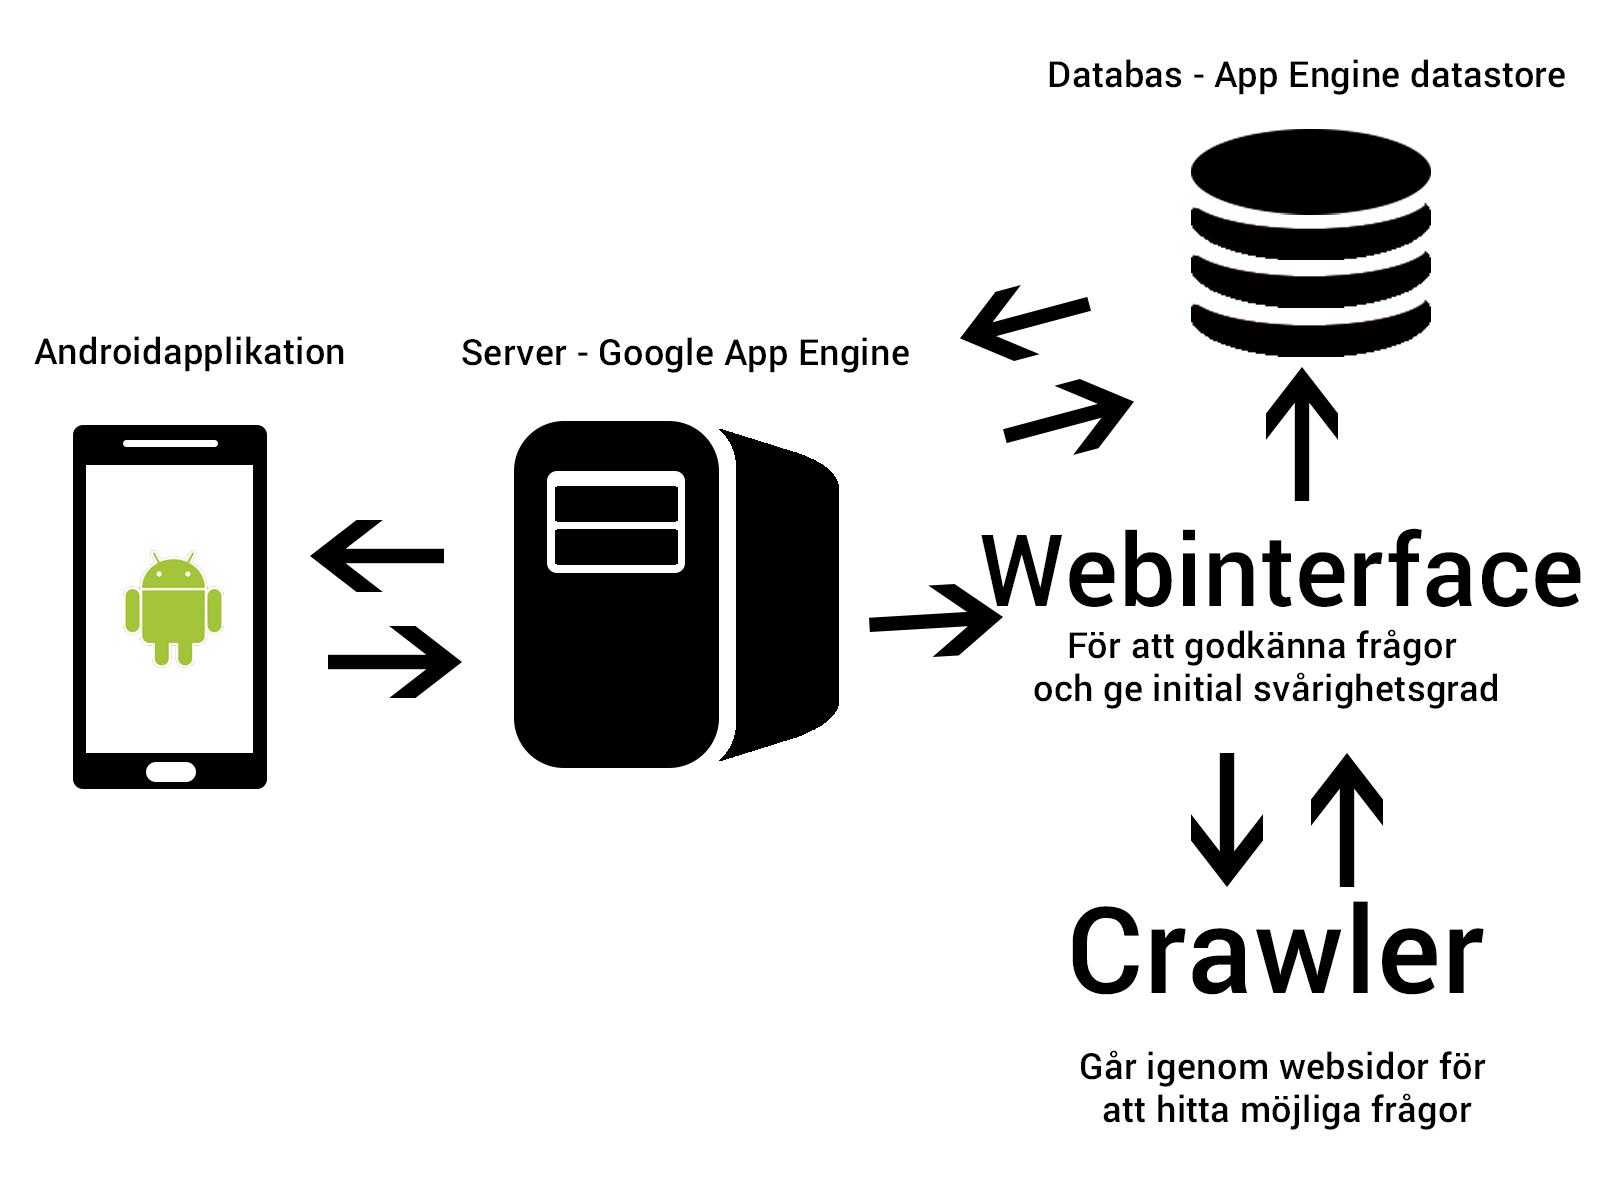
\includegraphics[width = \textwidth]{systemstruktur.jpg} 
	\end{centering}
	\caption{\textit{Illustration av systemstrukturen}}
\end{figure} 

\subsubsection{Androidapplikationen}
Androidapplikationen, vilket är klienten i systemet, är spelet som utvecklats. Det här är den del av systemet som användaren interagerar med båda visuellt och funktionellt.

När det är den aktuella spelarens tur får denne en chunk med fem frågor och dess svar (årtal). Det är sedan klienten som rättar frågorna och därefter skickas resultaten tillbaka till servern.
\subsubsection{Server}
Klienten kommunicerar med en server som körs i Google App Engine. Servern är utvecklad i programspråket Go (Golang) \cite{golang}. Servern agerar även som en brygga mellan klienten och den databas som används. När klienten kräver nya frågor till spelet kommunicerar servern med databasen som skickar frågorna till servern som i sin tur skickar vidare till klienten. Utöver kommunikation till klienten och databasen används även servern för att köra crawlern som är den automatiska informationshämtaren. Servern har också till uppgift att med jämna mellanrum köra fråge- och användarbalanseringssystemet som justerar svårighetsgraden på frågorna respektive spelarna i systemet. 
\subsubsection{Databas}
Databasen som servern kommunicerar med körs, likt servern, i App engine med biblioteket \textit{datastore}. Datastore är Google App Engines egna bibliotek för hantering av data där systemet hanterar datalagring med både SQL och noSQL.
\subsubsection{Crawler}
Inbyggt i servern finns en form av crawler som hanterar semi-automatisk informationshämtning av frågematerial. Hela systemet syftar till att via en given länk läsa igenom den länkade sidan och dess undersidor för att hitta information som passar som frågor för spelet. 

Sidor som har visat sig vara relativt enkla att läsa in är Wikipedias undersidor av typen listningssidor. Den här typen av sidor har en punktlista med årtal samt en beskrivande mening av det årtalet inom den kategori som Wikipediasidan handlar om. Ett exempel är sidan som listar datorspelsår: Som återfinns vid denna  \textbf{\href{http://sv.wikipedia.org/wiki/Lista_\%C3\%B6ver_datorspels\%C3\%A5r}{länk.}} 
Vid inläsning av den här typen av sida separeras helt enkelt varje $<$li$>$-element där ett bindestreck eller kolon förekommer och därefter sparas varje kombination av årtal och händelse i ett temporärt cache.

När alla  händelser har lästs in i cachet presenteras de inlästa händelserna en i taget i ett webinterface. Webinterfacet visar ett årtal, en fråga samt fyra knappar. Knapparna anger svårighetsgrad lätt, medel eller svår samt ett alternativ för att ta bort den aktuella frågan helt.

\begin{figure}[H]
	\begin{centering}
	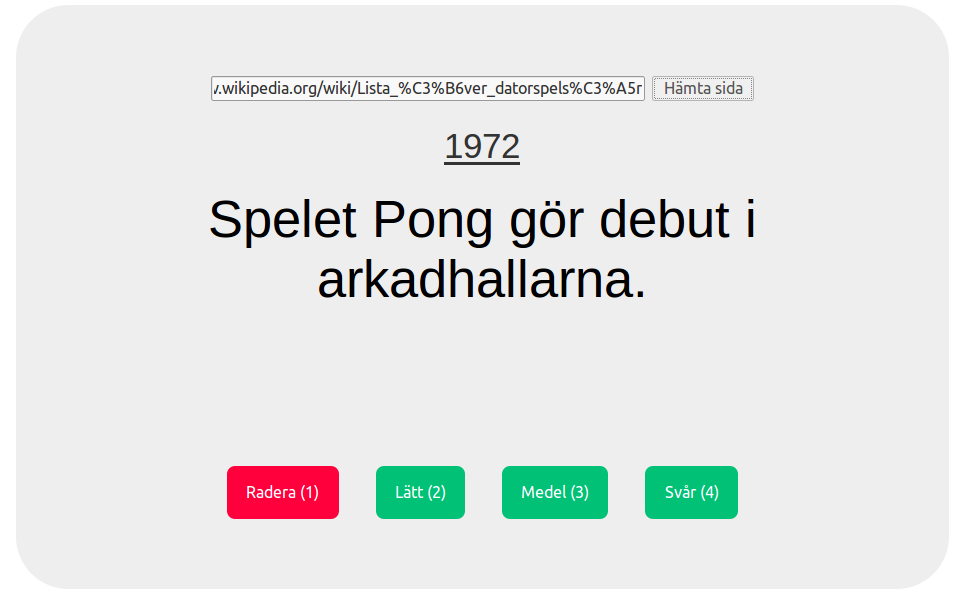
\includegraphics[width=\textwidth]{crawler} 
	\end{centering}
	\caption{\textit{Webinterface för crawlern}}
\end{figure}

De fyra knapparna är mappade till siffrorna 1-4 på tangentbordet för att det ska gå snabbt att klicka igenom frågorna. Texten är också redigerbar för att administratören snabbt ska kunna justera grammatiska fel.

\subsubsection{Användare}
Det finns två sorters användare som kan interagera med systemet.\\
\textbf{Administratörer} \label{admins} \\
Administratörerna är ansvariga för underhållet och utvecklingen av systemet. Administratörerna har den högsta typen av tillgång till systemet för att kunna utföra dessa uppgifter. I underhåll innefattas att felsöka och åtgärda funna fel men också uppföljning av rapporterade fel som skickas in av spelare. En vital uppgift som administratörerna har förutom den allmänna underhållet och utvecklingen av systemet är att godkänna informationen som hämtas av crawlern. Detta är för att se till att frågorna följer den struktur som administratörerna finner lämplig. \\
\textbf{Spelare}\\
Spelarna är den typen av användare som har en begränsad åtkomst till systemet. Spelarna kan endast komma åt systemet genom klienten och kan interagera med själva spelet. Detta betyder att en vanlig spelare inte kan finna information som ligger \textit{under huven} på systemet. Detta är delvis en säkerhetsåtgärd som är till för att den vanliga användaren inte, av misstag, eller med flit kunna komma åt systemets vitala delar och alternera dessa. Användaren kan kommunicera med administratörerna genom att skicka felrapporter om spelet skulle bete sig konstigt eller om några buggar har funnits.

\subsubsection{Balanseringssystemet}
Balanseringssystemet syftar till två saker, dels till att justera svårighetsgraden på frågorna som finns i databasen och dels till att justera spelarnas svårighetsnivå. 

Det finns alltså två separata nivåsystem i applikationen. Varje fråga i databasen har ett siffervärde för dess svårighetsgrad, ju högre siffra, desto svårare fråga. På liknande vis har också varje användare en svårighetsgrad som lagras som ett siffervärde i spelarens profil. Syftet med dessa poäng är i det stora perspektivet att få spelet att servera så rättvisa och roliga matcher som möjligt för spelarna. 

Frågornas svårighetsnivå justeras beroende på hur spelarna i matchen svarar på frågan. En fråga som det ofta svaras fel på ökar i svårighetsnivå allt eftersom fler spelare svarar fel. Svårighetsnivån är helt bunden till frågan i sig och finns alltså kvar mellan matcherna.

En frågas svårighetsnivå har ingenting med någon form av poängräkning att göra. Svårighetsnivån på frågorna finns till för att vid en matchstart kunna jämföras mot spelarnas svårighetsnivå, på så vis avgör spelet om frågan ska skickas till spelarna eller inte. Det handlar alltså helt och hållet om att spelet ska presentera frågor som är lagom svåra för spelarna, så att spelet blir lagom utmanande och maximalt roligt.

Spelarnas svårighetsnivåer justeras också efter avslutad match. Den här balanseringen går i stora drag till så att den vinnande spelaren tar poäng av den förlorande spelaren. Om den vinnande spelaren redan ligger på högre nivå än den förlorande så tar denne väldigt lite poäng från den förlorande. I det motsatta fallet tar istället den vinnande spelaren mycket poäng från den förlorande. Hur mycket poäng som faktiskt tas baseras på skillnaden i nivå mellan spelarna. 

Inspiration till den här sortens balansering kommer bland annat från Counter-strike: GO \cite{cs} som använder sig av ett system kallat Elo\cite{elo}. Elo är ett system som förutser hur stor del av en mängd spelade matcher som bör vinnas av vardera spelare, baserat på en den svårighetsnivå respektive spelare har. Det här systemet justerar, efter en match, poängen enligt beskrivningen ovan. Eftersom en lägre rankad spelare får fler poäng vid vinst mot en högre rättar systemet på sikt sig självt, vilket innebär att spelarna faktiskt får den nivå de förtjänar.

Elosystemet fungerar enligt följande. Varje spelare får en initial Elopoäng på 1000. Denna justeras sedan beroende på utfallet av en match i förhållande till det förväntade utfallet. Det förväntade utfallet beräknas:

$$E_A = \frac{1}{1+10^{(R_B-R_A)/400}}$$

Där $E_A$ är den förväntade andelen matcher som spelare A borde vinna. Är värdet till exempel 0.84 så innebär det att 84\% av matcherna borde vinnas av spelare A enligt nuvarande Elopoäng. $R_B$ är spelare B:s nuvarande Elopoäng och $R_A$ är spelare A:s nuvarande poäng.

När det förväntade utfallet har beräknats så justeras sedan spelarnas Elopoäng enligt formeln:

$$R'_A = R_A + K(S_A-E_A)$$

Där $R'_A$ är spelare A:s nya Elopoäng, $R_A$ är spelare A:s Elopoäng innan matchen, $S_A$ är det faktiska utfallet av matchen och $E_A$ är det förväntade utfallet. K-värdet är en skalningsfaktor som justerar hur mycket poängen justeras vid varje vinst/förlust.

Ett räkneexempel med spelare A, 1300 poäng, och spelare B 1000 poäng, där A vinner:

$$0.849 = \frac{1}{1+10^{(1000-1300)/400}}$$
$$ R'_A = 1300 + 16(1-0.849) = 1302.416 $$
$$ R'_B = 1000 + 16(0-0.849) = 997.584 $$

Efter varje avslutad match skickas alla frågor som var med i matchen samt båda spelarnas svar på respektive frågor. Utifrån detta justeras sedan nivåerna.

Om en spelare med låg nivå svarar rätt på en fråga så justeras frågans svårighetsgrad ner, ju högre nivå frågan har, desto större nedjustering sker. En spelare med hög nivå påverkar inte frågorna lika mycket som en spelare med låg nivå. Det här beror på att om en spelare med låg nivå svarar rätt på en svår fråga så är nivån på frågan förmodligen mycket mer felaktig än om en avancerad spelare svarat rätt på samma fråga. 

\begin{verbatim}
downDiff = int((1.0-(userRatio*questionRatio))*10.0)
\end{verbatim}

Kodsnutten ovan är ett exempel på en justering som sker om en spelare svarat rätt på den aktuella frågan. userRatio är ett värde mellan 0-1 på spelarens nivå (0 är nybörjare, 1 är avancerad). questionratio är ett värde mellan 0-1 på frågans nivå. downDiff är det värde som frågans nivå sänks med (mellan 0-10). 

\subsection{Avgränsningar}
Någon applikation för Windows och iOS fanns som en eventuell fortsatt utveckling efter Android men kommer inte att ske ty ett större fokus på en bra applikation till Android prioriteras. Spelet kommer troligtvis ha ett par kategorier för frågorna som ska finnas med i spelet, men dessa är ännu inte valda. 

I applikationen finns det många funktioner som skulle vara roliga och användbara, men inför projektet hade vi några funktioner som ansågs vara viktiga att ha med. Den viktigaste funktionen är att kunna hitta och spela en match. En funktion för att hitta och hantera vänner man har i spelet och även kunna se statistik över matcherna man spelat mot en vän. Dessa funktioner behöver så klart även implementeras på servern.

\subsection{Krav}
Systemet ska klara många spelare samtidigt, dock bara två per match. Någon speciell tak för antalet användare är inte bestämt ännu men med tanke på den otroligt solida grunden för skalbarhet som projektet står på kommer en siffra för antal spelare ganska snart kunna bestämmas. Eftersom App Engine används för servern så kommer det inte bli något problem med den enkla förklaringen att det är en tjänst som automatiskt skalar med hänsyn på belastning. \cite{appenginescalability}

Informationssökaren ska tillsammans med den administrativa kontrollen ge frågor som håller hög kvalitet. En hög kvalitet betyder frågor som är relevanta och som följer den strukturen vi har tänkt oss. Frågorna ska vara lätta att läsa, förstå och samtidigt befinna sig i det breda spektrumet av svårighetsgrader vi kommer ha i spelet. Sökaren för frågorna ska också vara så pass bra att den administrativa kontrollen går fort och att så lite som möjligt behöver korrigeras efter att frågorna har samlats in. För att applikationen inte ska kännas alldeles för repetitiv ska det finnas många frågor som dessutom är av varierande kategori. Det ska också finnas minst 1000 frågor sammanlagt.

Designen av applikationen är något som är väldigt viktigt för oss. Kravet i början var att ha en intuitiv, responsiv och snygg design. Eftersom applikationen gjordes för Android skulle den också följa dess designmönster Material Design \cite{MaterialDesign}.

\subsection{Utvärdering}
Planen är att en fungerande alfa eller betaversion av systemet ska färdigställas en rimlig tid innan projektet avslutas. I den här versionen ska användare ha möjlighet att ge feedback och att testa applikationen. Tack vare den feedback vi får från användarna så ska så många fel som möjligt justeras innan den skarpa versionen släpps.

Gränssnittet och användandet av applikationen kommer också att utvärderas med hjälp av think aloud \cite{thinkaloud} och en heuristic evaluering \cite{heruistic}.

\newpage
\printbibliography[title={Referenser}]
\end{document}